\subsection{Memory and bandwidth overheads}
\label{s:eval:traces}
\label{sec:eval:traces}

In this section, we answer the following questions:
\begin{CompactEnumerate}
\item What is a good size for the on-chip key value store?
\item What are the eviction rates to the backing store?
\item How accurate are queries that are not mergeable?
\end{CompactEnumerate}

\Para{Experimental setup.}  We simulate a \TheSystem query over three unsampled
packet traces: two traces from \tenglink core Internet routers, one from
Chicago (\textasciitilde{}150M packets) from 2016~\cite{caida2016} and one from
San Jose (\textasciitilde{}189M packets) from 2014~\cite{caida2014}; and a 2.5
hour university data-center trace (\textasciitilde{}100M packets) from
2010~\cite{bensonDC}. We refer to these traces as Core16, Core14, and DC
respectively.

We evaluate the impact of memory size on cache evictions for a \TheSystem query
that aggregates by \txtftuple.  As discussed in
\S\ref{sec:hardware-feasibility}, our hardware design uses an 8-way LRU cache.
We also evaluate two other geometries for the cache: a hash table, which evicts
the incumbent key upon a collision, and a fully associative LRU. Comparing our
8-way LRU with other hardware designs demonstrates the tradeoff between
hardware complexity and eviction rate.

\Para{Eviction ratios.}
Each evicted key-value pair is streamed to a backing store.  This requires the
backing store to process packets as quickly as they are evicted, which depends
on the incoming packet rate and the eviction ratio, \ie the ratio of evicted
packets to incoming packets.  The eviction ratio depends on the geometry of the
on-chip cache, the packet trace, and the cache size (\ie the number of
key-value pairs it stores). Hence, we measure eviction ratios over (1) the
three geometries for the Core16 trace (Figure~\ref{fig:eviction-geo}), (2) the
three traces using the 8-way LRU geometry (Figure~\ref{fig:eviction-traces}),
and (3) for caches sizes between $2^{16}$ (65K) and $2^{21}$ (2M) key-value
pairs.

% resume here

\begin{figure}[!t]
\centering
\begin{subfigure}[t]{0.48\columnwidth}
\raggedright
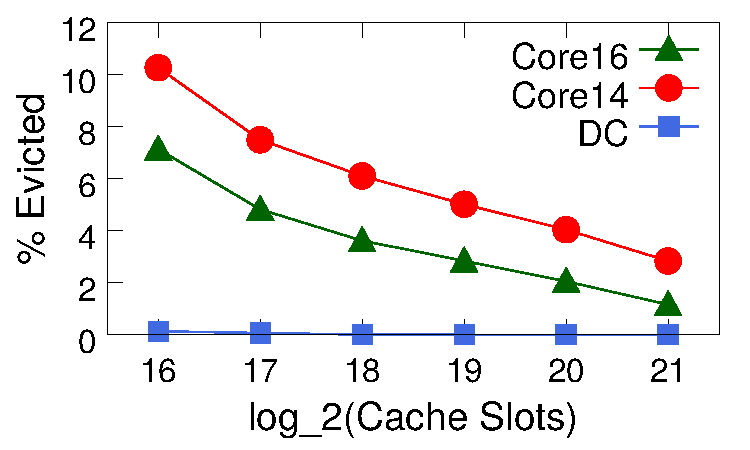
\includegraphics[width=\linewidth]{pq_eviction-rate-alltraces.pdf}
\vspace{-0.2in}
\caption{By trace}
\label{fig:eviction-traces}
\end{subfigure}
\begin{subfigure}[t]{0.48\columnwidth}
\raggedleft
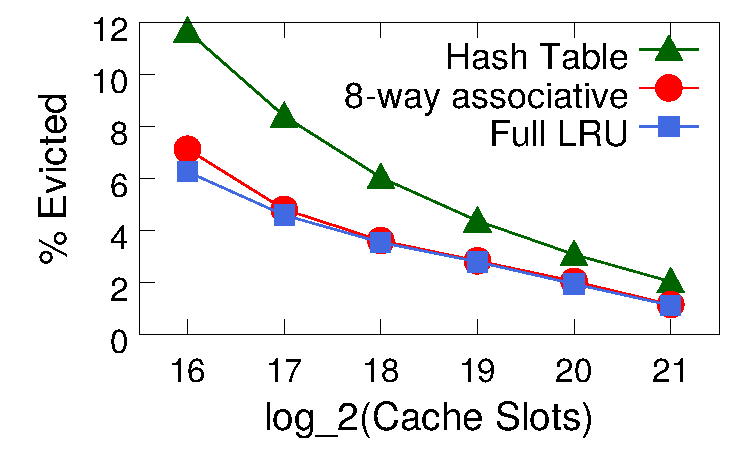
\includegraphics[width=\linewidth]{pq_eviction-rate-geo-core16.pdf}
\vspace{-0.2in}
\caption{By cache geometry (Core16)}
\label{fig:eviction-geo}
\end{subfigure}
\vspace{-0.1in}
\caption{Eviction ratios to the backing store.}
\vspace{-0.25in}
\label{fig:eviction-ratios}
\end{figure}

\Fig{eviction-geo} shows that a full LRU has the lowest eviction ratios, since
the entire LRU must be filled before an eviction occurs. However, the 8-way
associative cache is a good compromise: it avoids the hardware complexity of a
full LRU while coming within 2\% of its eviction ratio.  \Fig{eviction-traces}
shows that the DC trace has the lowest eviction ratios.  This is because it has
much fewer unique keys than the other two traces and these keys are less likely
to be evicted.

The reciprocal of the eviction ratio (as a fraction) is the reduction in server
data collection load relative to a {\em per-packet collector} that processes
per-packet information from routers. For example, for the Core14 trace with a
$2^{19}$ key-value pair cache, the server load reduction is 25$\times$
(corresponding to an eviction ratio of 4\%).

\Para{Eviction rates.}
Eviction ratios are agnostic to specifics of the router, such as link speed,
link utilization, and on-chip cache size in bits. To translate
eviction ratios (evictions per packet) to eviction \emph{rates} (evictions per
second), we first compute the average packet size (700 Bytes) and link utilization
(30\%) from the Core16 trace.

Next, we estimate the on-chip cache size for a \tengrouter router and a
\hundredgrouter router.
On a \tengrouter router, SRAM
densities are $\approx$ 3--4 $\nicefrac{Mbit}{mm^2}$~\cite{sram_45nm_wiki}, and
the smallest router chips occupy 200
\si{\milli\metre\squared}~\cite{gibb_parsing}.  Therefore, a 64 Mbit cache in
SRAM costs around 10\% additional area, which we believe is reasonable.
For recent \hundredgrouter routers~\cite{tomahawk2},
 SRAM densities are $\approx7
\nicefrac{Mbit}{mm^2}$~\cite{sram_estimate}, and the routers occupy
$\approx$ 500 \si{\milli\metre\squared},\footnote{S. Chole. Cisco Systems. Private
communication.  June 2017.} making a 256 Mbit cache (7.3\% area
overhead) a reasonable target.

For a given query, we divide these cache sizes by the size of
the aggregation's key-value pair to get
the number of key-value pairs. We then look up this number in \Fig{eviction-ratios}
to get the eviction ratio for that query, which we translate to an eviction rate
using the network utilization and packet size mentioned earlier.

Eviction rates for some sample queries are shown in \Fig{evt-rate-queries}.
 For a \tengrouter router with a 64 Mbit cache, we observe eviction rates of
$\approx$ 1M packets per second.  For a \hundredgrouter router with a 256 Mbit
cache and the same average packet size and utilization, the eviction rates can
reach
 7.17M packets per second. Relative to a per-packet collector,
\TheSystem reduces the server load by 25--80$\times$.

The eviction rates for both the \tenglink and \hundredglink routers are
under 10M packets per second, well within the capabilities of multi-core
scale-out key-value
stores~\cite{redis_benchmark, memcached_benchmark, redis_vs_memcached_update},
which typically handle 100K--1M operations per second per core.  For instance,
for a single \tengrouter router running an aggregation with a 64-bit
state size, a single 8-core server is sufficient to handle the eviction rate of
1.08M packets per second. For a single \hundredgrouter router running
the same aggregation, the eviction rate goes up to 5.18M packets per
second, requiring four such servers.

\begin{figure}[!t]
\centering
\resizebox{0.5\textwidth}{!}{
%%\begin{tabular}{p{0.15\textwidth} p{0.06\textwidth} p{0.093\textwidth} p{0.093\textwidth} }\hline
\begin{tabular}{llll}\hline
%% {\small \textbf{Query}} & {\small \textbf{State size (bits)}} & {\small
%%   \textbf{Eviction rate at \tenglink (pkts/s)}} & {\small \textbf{Eviction rate
%%     at \hundredglink (pkts/s)}}\\ \hline \hline
  {\textbf{Query}} &
  {\textbf{State size}} &
  {\textbf{Eviction rate at}} &
  {\textbf{Eviction rate at}} \\

  &
  {\textbf{(bits)}} &
  {\textbf{\tengrouter}} &
  {\textbf{\hundredgrouter}} \\

  &
  &
  {\textbf{(packets/s)}} &
  {\textbf{(packets/s)}} \\

  \hline
  \hline
  
Packet count & 32 & 1.0M (34$\times$) & 4.29M (81$\times$) \\ \hline %2.91,1.24 
Lossy connections\nop{\footnote{Lossy Connections requires two stages that count
    by \txtftuple, which we consider as a single key-value store with a concatenated value.}}& 64  & 1.08M (32$\times$) & 5.18M (66$\times$) \\ \hline % 3.14, 1.51 
TCP out-of-sequence & 128 & 1.21M (28$\times$) & 6.72M (52$\times$) \\ \hline % 3.57,1.93
Flowlet size & 160 & 1.26M (27$\times$) & 7.17M (48$\times$) \\ 
histogram (Stage 1) & & & \\ \hline %3.66, 2.08
\end{tabular}
}
\vspace{-0.05in}
\caption{Eviction rates and reduction in collection server
  load for queries from \Fig{example-perf-queries}.
Each key-value pair occupies the listed state size plus 104 bits for a
\txtftuple key.
The 10-Gbit/s and 100-Gbit/s routers have a 64 Mbit and 256 Mbit cache, respectively.}
\label{fig:evt-rate-queries}
\vspace{-0.15in}
\end{figure}

\Para{Generalizing to other scenarios.}
\Fig{eviction-ratios} also generalizes to multiple aggregations and aggregations
of different state sizes. 
First, coarsening the
aggregation key by picking a subset of the \txtftuple reduces the eviction
ratio, since there are fewer keys in the working set. We believe that the
\txtftuple may well be the most fine-grained and still practically useful
aggregation level; hence, our results show the worst-case eviction ratios for a
single {\ct groupby}.  Second, variations in the size of the {\ct groupby}
value simply result in a different number of key-value pairs for a given memory
size. Third, running multiple {\ct groupby} queries with the same number of
key-value pairs, and aggregating by the same key, results in synchronized
evictions across all queries. Hence, the eviction rate can be read off
\Fig{eviction-ratios} at the correspondingly reduced memory size.
%TODO: Maybe the above can be improved.

%%Hence, given an aggregation function, the corresponding eviction rate
%%(in packets per second) can be determined by using the total key-value size to
%%determine the number of available key-value pairs and then interpolating the
%%curves in \Fig{eviction-traces}

\Para{Accuracy of non-mergeable queries.}
Queries that are neither linear-in-state nor associative cannot be merged in
the backing store. If a key from such a query is evicted multiple times,
\TheSystem cannot guarantee its correctness and marks it as invalid. However,
these keys' values are still valid if they are either never evicted or are
evicted once and never reappear. We quantify a query's accuracy as the
fraction of keys with valid values over the query's lifetime.
\Fig{accuracy-traces} shows query accuracy using the three traces, with the DC
trace being near-perfect since it has fewer unique keys, and hence, evictions.
If the query is run over a shorter time interval, its accuracy is typically
higher, since the cache may not be full and a smaller fraction of keys are
evicted.  \Fig{accuracy-time} shows this tradeoff for a range of cache sizes
and geometries using the Core16 trace.  Shortening the query from 5 minutes to
1 minute boosts accuracy by 10\%.

\begin{figure}[ht]
\centering
\vspace{-0.1in}
\begin{subfigure}[t]{0.48\columnwidth}
\raggedright
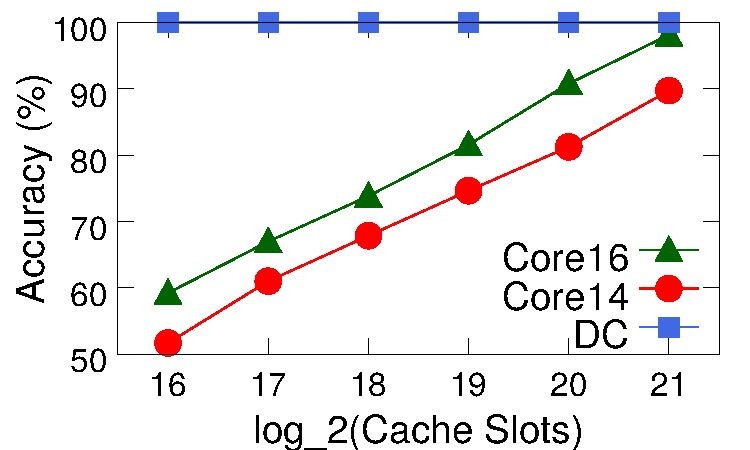
\includegraphics[width=\linewidth]{pq_accuracy-alltraces.pdf}
\caption{By trace}
\label{fig:accuracy-traces}
\end{subfigure}
\begin{subfigure}[t]{0.48\columnwidth}
\raggedleft
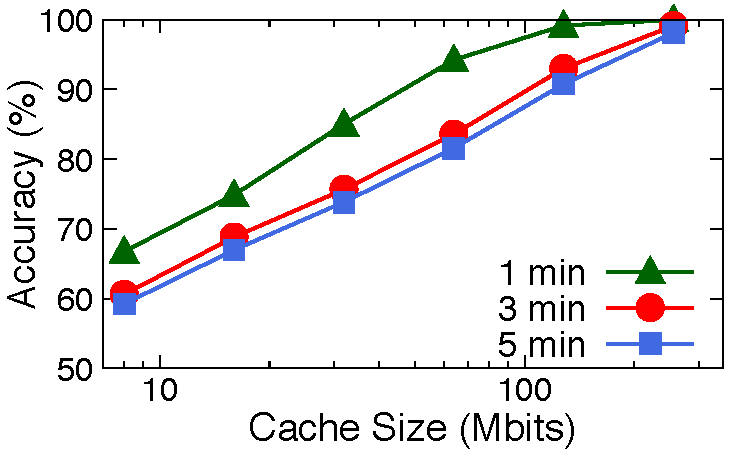
\includegraphics[width=\linewidth]{pq_accuracy-core-geo.pdf}
\caption{By query duration (Core16)}
\label{fig:accuracy-time}
\end{subfigure}
\vspace{-0.1in}
\caption{Query accuracy for non-mergeable aggregations.}
\end{figure}
